% Source of ACSF2605371_paper_zh_extended.pdf. Build in this folder with two runs of
%   xelatex -jobname=ACSF2605371_paper_zh_extended main.tex
% (fonts: TeX Gyre Termes/Heros, STIX Two Math, Noto Serif CJK SC) and copy ACSF2605371_paper_zh_extended.pdf to ../
\documentclass[a4paper,11pt]{article}
\usepackage{fontspec}
\setmainfont{TeX Gyre Termes}
\setsansfont{TeX Gyre Heros}
\newfontfamily\cjkfont{Noto Serif CJK SC}
\usepackage{amsmath}
\usepackage{unicode-math}
\setmathfont{STIXTwoMath-Regular.otf}
\usepackage[a4paper,top=2.5cm,bottom=2.4cm,left=2.6cm,right=2.6cm]{geometry}
\usepackage{graphicx,booktabs,array,threeparttable,pdfpages,fancyhdr,xurl}
\usepackage[font=small,labelsep=period,skip=4pt]{caption}
\usepackage[hidelinks,bookmarksnumbered=true,bookmarksopen=true]{hyperref}
\usepackage{titlesec}
\renewcommand{\floatpagefraction}{0.8}\renewcommand{\topfraction}{0.88}\renewcommand{\bottomfraction}{0.7}\renewcommand{\textfraction}{0.1}
\usepackage{etoolbox}\AtBeginEnvironment{thebibliography}{\small\linespread{1.05}\selectfont\setlength{\itemsep}{1pt}\setlength{\parskip}{0pt}}
\setlength{\emergencystretch}{3em}
\linespread{1.15}
\setlength{\parskip}{0.25em}
\titleformat{\section}{\large\bfseries}{E\arabic{section}}{0.8em}{}
\titleformat{\subsection}{\normalsize\bfseries}{E\arabic{section}.\arabic{subsection}}{0.6em}{}
\renewcommand{\thesection}{E\arabic{section}}
\renewcommand{\thefigure}{E\arabic{figure}}
\renewcommand{\thetable}{E\arabic{table}}
\renewcommand{\theequation}{E\arabic{equation}}
\setlength{\headheight}{15pt}\pagestyle{fancy}\fancyhf{}\renewcommand{\headrulewidth}{0.4pt}
\newcommand{\hd}[1]{\begin{tabular}[b]{@{}c@{}}#1\end{tabular}}
\newcommand{\exthead}[1]{\fancyhead[L]{\small #1}\fancyhead[R]{\small Part II\quad Post-competition extensions}\fancyfoot[C]{\small E-\thepage}}

\graphicspath{{../../figures/extension/}}
\hypersetup{pdftitle={Multi-energy transition under construction lags and repeated shocks -- extended edition}}
\begin{document}
\thispagestyle{empty}
\begin{center}
{\Large\bfseries Multi-Energy Transition under Construction Lags and Repeated Shocks:\\[0.2em] Multi-Agent Simulation and Security-Constrained Optimisation}\\[0.7em]
{\large Extended edition --- note}
\end{center}
\vspace{0.8em}

This file has two parts. Part I is the paper submitted to Problem A of the National College Student Simulation Modeling Application Challenge, 2026 (57 pages, in Chinese), reproduced exactly as submitted. Part II, starting on page E-1, contains post-competition extensions written in November 2026.

The model is calibrated on statistics for 2010--2024. Its first simulated year, 2025, is fixed uniquely by the state of 2024 and the construction queue and does not depend on the investment plan, so the official 2025 statistics published afterwards allow a genuine out-of-sample test. E1 shows that energy totals, the energy mix and slowly changing capacities are reproduced within about 1.4\,\%, while wind and solar capacity are under-predicted by 8.5\,\% and 10.1\,\%. E2 traces this deviation to the throughput of the initial construction pipeline rather than to the construction lag, and re-anchors the model to the actual throughput of 2025. Remaining net emissions in 2060 fall by 7.3\,\% in the baseline scenario, but because the annual investment budget binds in all 36 years, cumulative unserved useful service rises 2.7-fold. The paper's central trade-off between the speed of the transition and the security of supply is therefore reinforced rather than overturned.

Every number in Part II can be reproduced with the scripts in the \texttt{extension/} folder of the code repository; result files are in \texttt{results/extension/}, and the sources of the 2025 statistics are listed in the scripts.

\clearpage
\pdfbookmark[0]{Part I\quad Competition paper (as submitted)}{part1}
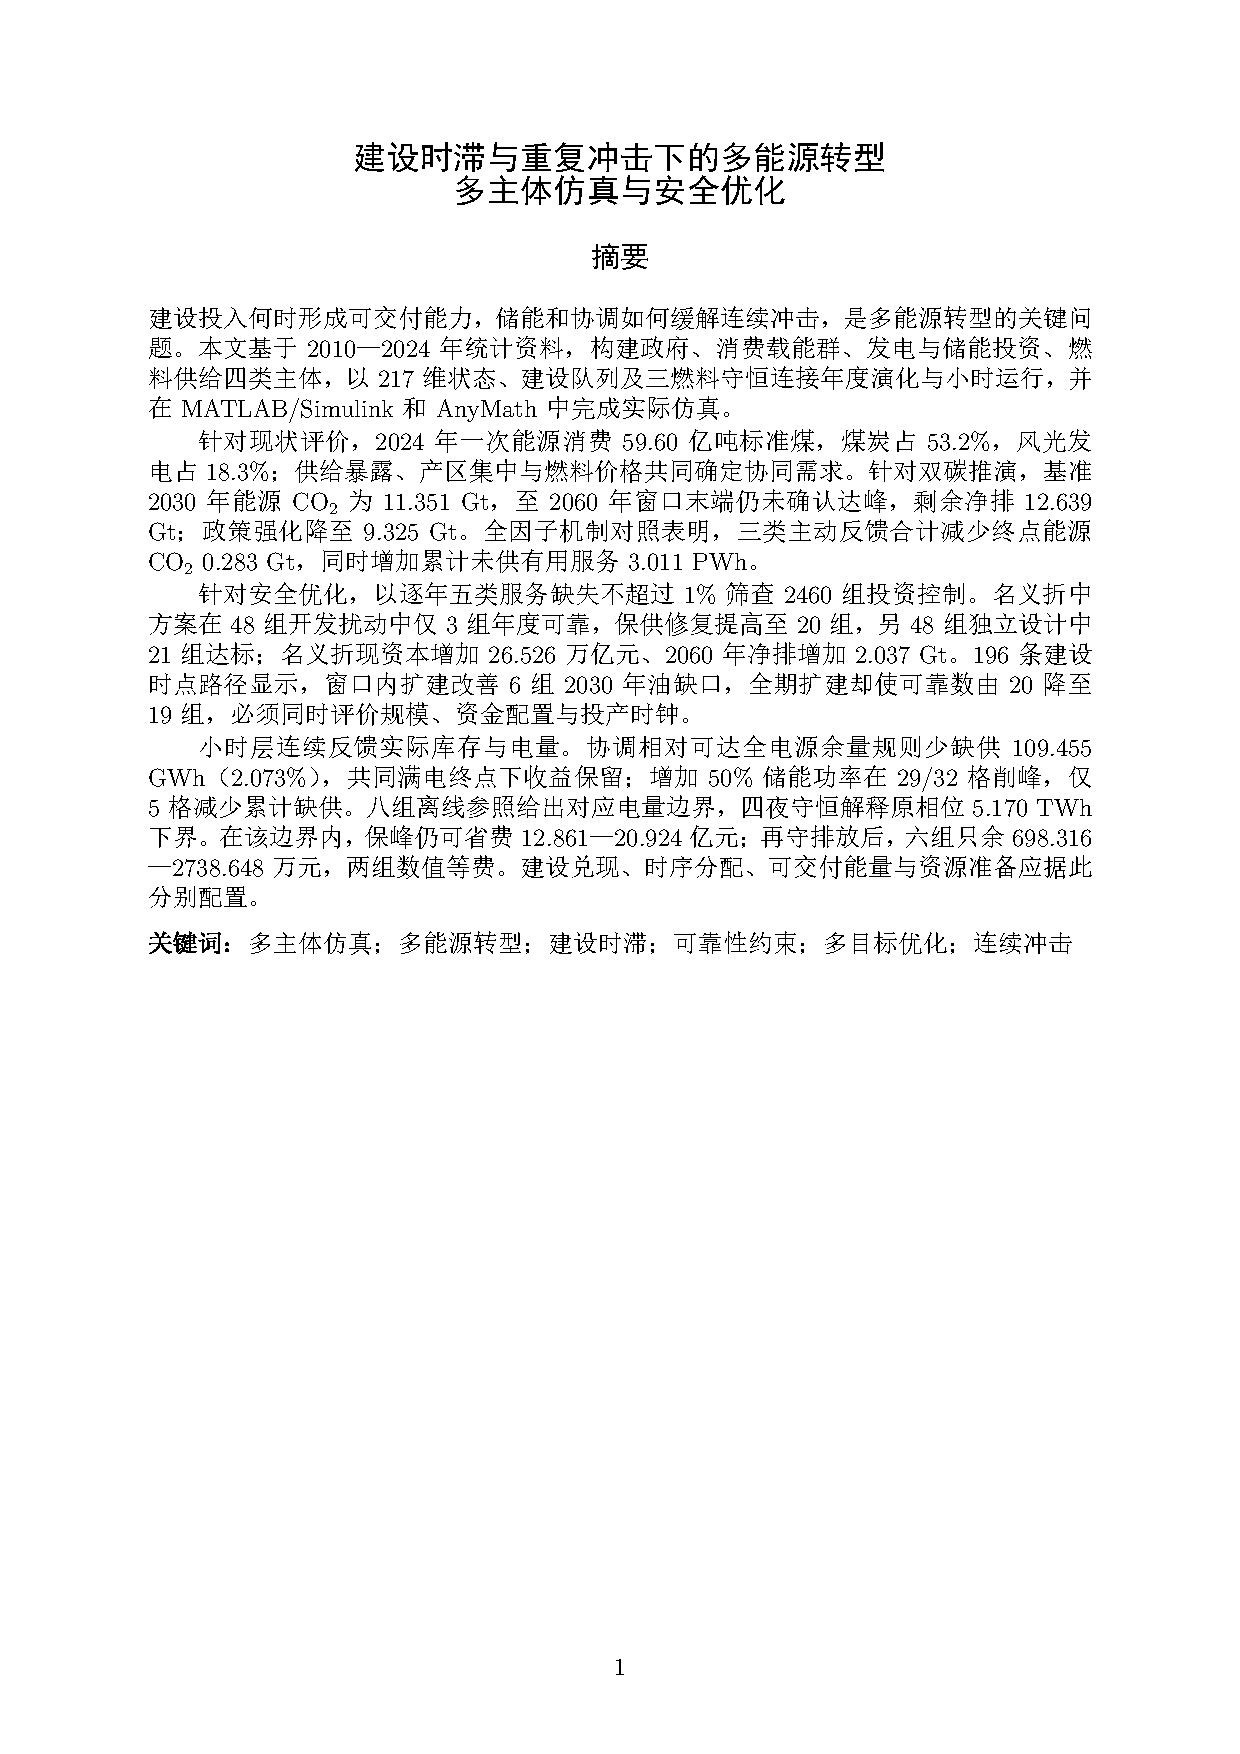
\includepdf[pages=-]{../ACSF2605371_paper_zh.pdf}
\pdfbookmark[0]{Part II\quad Post-competition extensions}{part2}
\setcounter{page}{1}
\exthead{Multi-energy transition under construction lags and repeated shocks}
\begin{center}{\Large\bfseries Part II\quad Post-competition extensions}\end{center}

The paper builds a multi-energy transition model with four kinds of agents, the government, energy-using sectors, generation and storage investors, and fuel supply, and carries out dual-carbon scenarios, security-constrained investment optimisation and recovery from repeated shocks on an annual and an hourly scale. The parameters are calibrated on statistical yearbook data for 2010--2024. The official statistics for 2025 were published only after the paper was completed, which provides a year that no parameter of the model has seen.

\section{Can the model predict 2025? An out-of-sample test}

\subsection{Design}
The first simulated year of the model is fixed uniquely by the state of 2024 and the construction queue and is identical under every investment plan, so the simulated values for 2025 are a forecast that does not depend on the choice of plan. E1 compares them item by item with the statistical communiqué of the National Bureau of Statistics published on 28 February 2026, the supplementary energy-mix data published in June 2026 and the electricity statistics of the National Energy Administration. Thermal capacity is not compared, because the statistical category ``thermal power'' also contains oil-fired and waste-to-energy units that the model does not include.

\subsection{Results}
\begin{table}[htbp]\centering\small
\caption{Simulated values for 2025 against official statistics.}\label{tab:sim-e1}
\begin{tabular}{lrrr}\toprule
Indicator (2025) & Model & Statistics & Error\\\midrule
Primary energy consumption (Mtce) & 6122 & 6170 & $-0.8\,\%$\\
Electricity demand vs. total consumption (TWh) & 10493 & 10368 & $+1.2\,\%$\\
Non-fossil share of primary energy & 22.0\,\% & 21.7\,\% & $+0.3$ pp\\
Hydro capacity incl. pumped storage (GW) & 444 & 448 & $-1.0\,\%$\\
Nuclear capacity (GW) & 63.4 & 62.5 & $+1.4\,\%$\\
Wind capacity (GW) & 585 & 640 & $\mathbf{-8.5\,\%}$\\
Solar capacity (GW) & 1080 & 1202 & $\mathbf{-10.1\,\%}$\\\bottomrule
\end{tabular}
\end{table}

\begin{figure}[htbp]\centering
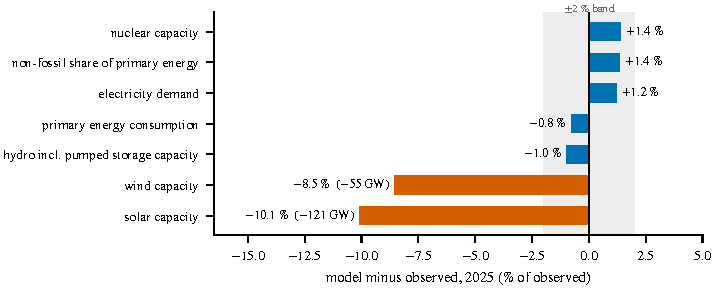
\includegraphics[width=0.62\textwidth]{figE1_holdout_2025.pdf}
\caption{Error of the simulated 2025 values relative to official statistics. The non-fossil share is plotted as the relative error of the share itself ($+1.4\,\%$), which corresponds to $+0.3$ percentage points.}\label{fig:sim-e1}
\end{figure}

Energy totals, the energy mix and slowly changing capacities are reproduced within about 1.4\,\% (Table~\ref{tab:sim-e1}, Figure~\ref{fig:sim-e1}), but the construction queue under-delivers the record wind and solar additions of 2025, by 55 GW and 121 GW respectively. The next section traces this residual to its source and follows its consequences through to the conclusions of the paper.

\section{What the 2025 deviation identifies, and what correcting it changes}

\subsection{Source of the deviation}
In the model, capacity in 2025 equals capacity in 2024 plus the first deliveries of the initial construction pipeline. The paper estimates this pipeline from steady throughput, the mean net additions of 2022--2024: 64 GW a year for wind (37, 76 and 79 GW in the three years) and 193 GW a year for solar (86, 217 and 277 GW). New orders need at least a year to be delivered, so the construction lag cannot affect 2025. E2 makes controlled changes to the Python implementation of the submitted annual core, whose native run reproduces the stored contest metrics exactly.

The residual identifies the throughput, not the construction lag (Figure~\ref{fig:sim-e2}a). Lengthening the construction lag of new orders by a factor of 1.5 or 2 leaves the 2025 capacity unchanged (585 GW of wind, 1080 GW of solar), whereas changing the throughput estimate moves the 2025 capacity one for one. Information available at the start of 2025 would already have improved the forecast: with the throughput of 2024 alone, the errors for wind and solar fall to $-6.1\,\%$ and $-3.1\,\%$, and the mean absolute deviation falls from 88 GW to 38 GW, whereas the linear trend of 2022--2024 over-predicts solar ($+5.8\,\%$).

\subsection{Consequences of the correction}
The same throughput also enters the investors' reference build path, so E2 anchors the model at both places to the actual throughput of 2025 and compares the baseline results of the paper (Table~\ref{tab:sim-e2}).

\begin{table}[htbp]\centering\small
\caption{Baseline results before and after anchoring to the actual throughput of 2025.}\label{tab:sim-e2}
\begin{tabular}{lrrr}\toprule
Baseline result & Paper & Anchored to 2025 & Change\\\midrule
Energy CO$_2$ in 2030 (Gt) & 11.351 & 11.017 & $-2.9\,\%$\\
Remaining net CO$_2$ in 2060 (Gt) & 12.639 & 11.713 & $-7.3\,\%$\\
Cumulative unserved useful service 2025--2060 (PWh) & 35.4 & 96.1 & $\times 2.7$\\\bottomrule
\end{tabular}
\end{table}

Correcting only the 2025 pipeline, with the reference path left as in the paper, changes the remaining emissions in 2060 by only about $-0.04$ Gt. The paper's qualitative findings hold in every variant: the baseline has no emissions peak before 2060, and under every throughput estimate the remaining emissions of the policy scenario in 2060 stay within 9.32--9.42 Gt (paper: 9.325 Gt). Only a longer construction lag raises them, to 9.48 Gt (factor 1.5) and 9.72 Gt (factor 2).

\begin{figure}[htbp]\centering
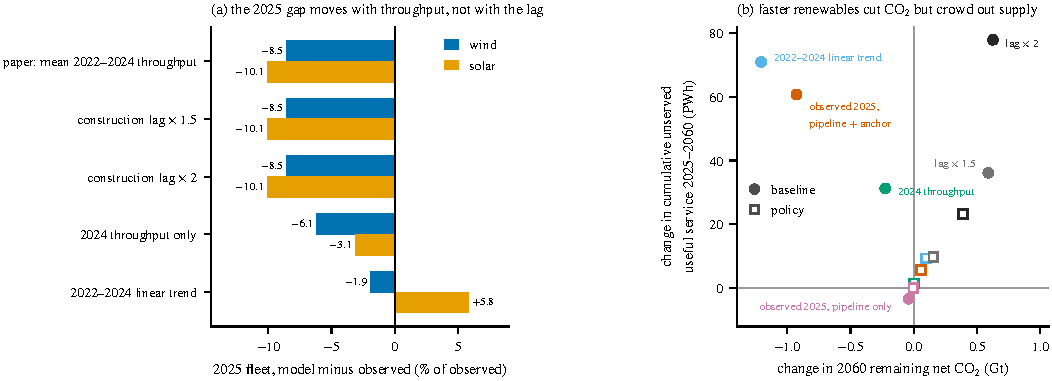
\includegraphics[width=\textwidth]{figE2_pipeline_recalibration.pdf}
\caption{(a) Error of the 2025 capacity under three estimates of the initial pipeline throughput and under two longer construction lags of new orders. (b) Change in remaining net CO$_2$ in 2060 and in cumulative unserved useful service relative to the paper's run; filled markers: baseline, open markers: policy scenario.}\label{fig:sim-e2}
\end{figure}

\subsection{Mechanism}
The annual investment budget binds in all 36 simulated years, so a faster reference path for renewables reallocates capital rather than adding to it. After anchoring to 2025, cumulative wind and solar investment in the baseline rises from 44.3 to 49.7 trillion CNY, investment in firm generation falls from 17.9 to 15.8 trillion CNY, and investment in fuel supply from 7.7 to 4.4 trillion CNY. As a result, unserved direct fuel demand rises from 4\,789 to 12\,635 Mtce and unserved electricity from 2\,546 to 9\,663 TWh. A longer construction lag raises both the remaining emissions in 2060 and the unserved service (Figure~\ref{fig:sim-e2}b).

\subsection{Conclusions and limits}
The 2025 statistics reinforce rather than overturn the paper's central trade-off: faster delivery of renewables lowers emissions but, under a shared budget, increases supply shortfalls unless supply-side investment is funded separately. The paper's estimate of the near-term renewable trajectory was conservative, and for a world that builds renewables at the pace of 2025 its security conclusions are, if anything, optimistic. Only one out-of-sample year is tested, and the conclusions depend on the modelling assumption of an annual investment budget; if the budget expanded endogenously with the pace of construction, the crowding-out of capital would be correspondingly smaller.
\end{document}
